\documentclass{article}
\usepackage[utf8]{inputenc}
\setlength\parindent{0pt}
\usepackage{nopageno}
\usepackage{amsmath}
\usepackage{amsfonts}
\usepackage{amssymb}
\usepackage{comment}
\usepackage{natbib}
\usepackage{graphicx}
\usepackage{float}
\usepackage{mathtools}
\usepackage{caption}

\title{Derivation of the Power Equation}
\date{}
\begin{document}
\maketitle

By the central limit theorem,
\begin{align*}
\frac{\bar{x} - \mu_0}{\sigma/\sqrt{n}}  \sim Z\ \big|\ \text{H}_0 \\
\frac{\bar{x} - \mu_A}{\sigma/\sqrt{n}}  \sim Z\ \big|\ \text{H}_A
\end{align*}

where $Z$ is distributed standard normal. Rearranging:

\begin{align*}
\bar{x} &\sim \frac{\sigma}{\sqrt{n}}Z + \mu_0\ \big|\ \text{H}_0 \\
\bar{x} &\sim \frac{\sigma}{\sqrt{n}}Z + \mu_A\ \big|\ \text{H}_A
\end{align*}

Without loss of generality, let $\mu_A > \mu_0$. The situation looks like this:

\begin{figure}[H]
    \centering
    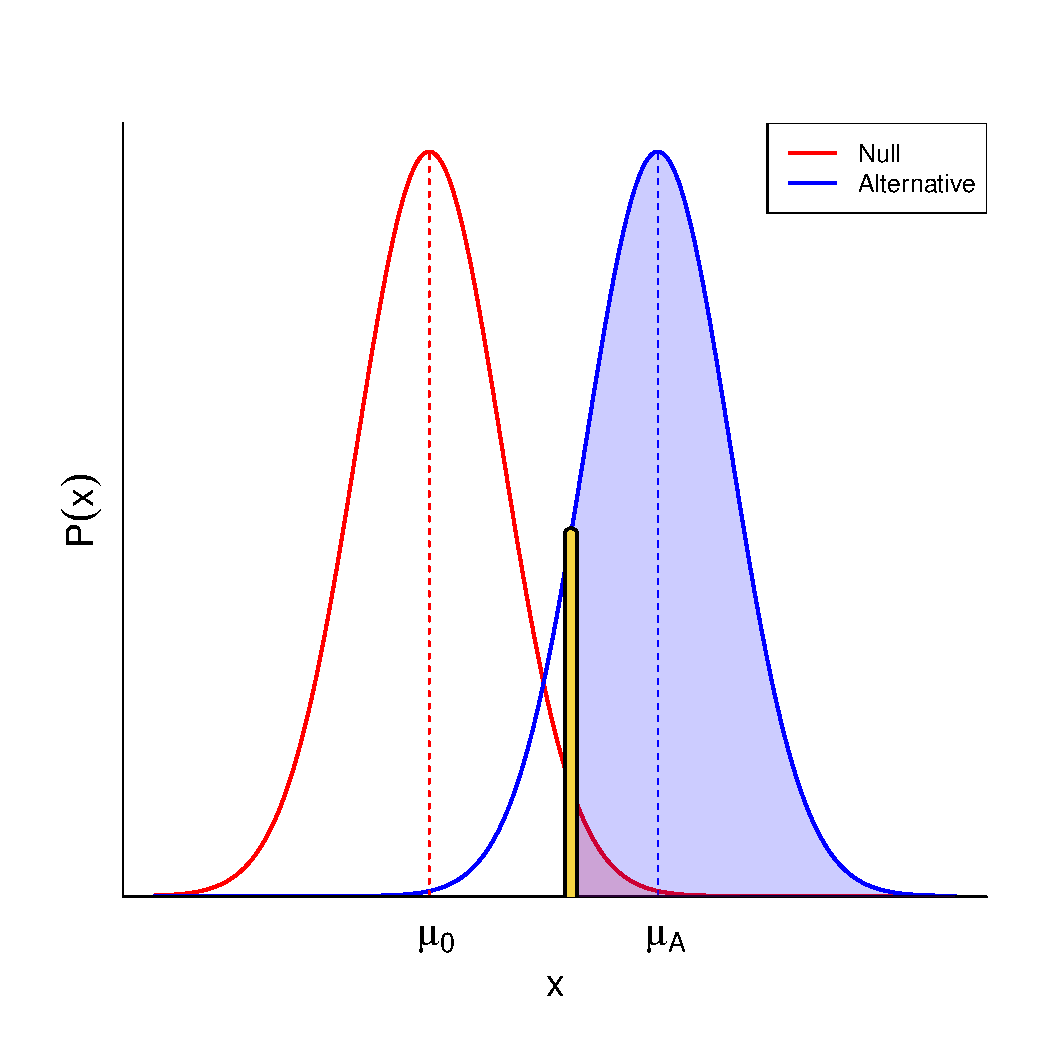
\includegraphics[width=0.7\linewidth]{normals.pdf}
    \caption*{The shaded regions are where the null is rejected under the two hypotheses.}
\end{figure}

We want to find the $x$-value where the yellow line is. Let's call it $Z_c$. We want $Z_c$ to satisfy the two properties:

\begin{align*}
\mathbb{P}(\bar{x} < Z_c \big|\ \text{H}_0) &= 1 - \alpha\\
\mathbb{P}(\bar{x} < Z_c \big|\ \text{H}_A) &= \beta
\end{align*}

These are met respectively when the following two equations hold:

\begin{align*}
Z_c &= \mu_0 + \frac{\sigma}{\sqrt{n}}Z_{1 - \alpha} \\
Z_c &= \mu_A + \frac{\sigma}{\sqrt{n}}Z_{\beta} = \mu_A - \frac{\sigma}{\sqrt{n}}Z_{1 - \beta}
\end{align*}

Because both are equal to $Z_c$, we can drop it and set the two right-hand side expressions as equal:

\begin{align*}
\mu_0 + \frac{\sigma}{\sqrt{n}}Z_{1 - \alpha} = \mu_A - \frac{\sigma}{\sqrt{n}}Z_{1 - \beta}
\end{align*}

Solving for $n$, we have:

\begin{align*}
\mu_A - \mu_0 &= \frac{\sigma}{\sqrt{n}}\big[Z_{1 - \alpha} + Z_{1 - \beta}\big] \\
\Rightarrow\quad \Aboxed{n &= \left[\frac{\sigma(Z_{1 - \alpha} + Z_{1 - \beta})}{\mu_A - \mu_0}\right]^2} \\
\end{align*}

The different flavors of power calculation come from:

\begin{itemize}
\item two-sided tests (just substitute $Z_{1-\alpha/2}$ in place of $Z_{1-\alpha}$)
\item hypothesis testing using a more complicated statistic, like $\bar{x}_1-\bar{x}_2$
\item using a different finite-sample approximation for the distribution of $\bar{x}$.
\end{itemize}


\end{document}
